\documentclass[12pt,letterpaper]{article}
\usepackage[utf8]{inputenc}
\usepackage[spanish]{babel}
\usepackage{graphicx}
\usepackage[left=2cm,right=2cm,top=2cm,bottom=2cm]{geometry}
\usepackage{graphicx} % figuras
\usepackage{hyperref}
% \usepackage{subfigure} % subfiguras
\usepackage{float} % para usar [H]
\usepackage{amsmath}
%\usepackage{txfonts}
\usepackage{stackrel} 
\usepackage{multirow}
\usepackage{enumerate} % enumerados
\renewcommand{\labelitemi}{$-$}
\renewcommand{\labelitemii}{$\cdot$}
% \author{}
% \title{Caratula}
\begin{document}

% Fancy Header and Footer
% \usepackage{fancyhdr}
% \pagestyle{fancy}
% \cfoot{}
% \rfoot{\thepage}
%

% \usepackage[hidelinks]{hyperref} % CREA HYPERVINCULOS EN INDICE

% \author{}
\title{Caratula}

\begin{titlepage}
	\begin{center}
	
	\begin{figure}[htb]
	\begin{center}
	
\includegraphics[width=4cm]{./Imagenes/UPT}
	\end{center}
	\end{figure}
	\vspace*{0.15in}
	\large{UNIVERSIDAD PRIVADA DE TACNA}\\
	\vspace*{0.10in}
	\large{Facultad de Ingeniería}\\
	\vspace*{0.10in}
	Escuela Profesional de Ingeniería de Sistemas  \\
	
	\vspace*{0.5in}
	\begin{large}
	TITULO:\\
	\end{large}
	
	\vspace*{0.1in}
	\begin{Large}
	\textbf{Práctica de Laboratorio N° 01: \\ Modelamiento Dimensional} \\
	\end{Large}
	
	\vspace*{0.3in}
	\begin{Large}
	\textbf{Curso:} \\
	\end{Large}
	
	\vspace*{0.1in}
	\begin{large}
	INTELIGENCIA DE NEGOCIOS\\
	\end{large}
	
	\vspace*{0.3in}
	\begin{Large}
	\textbf{Docente:} \\
	\end{Large}
	
	\vspace*{0.1in}
	\begin{large}
	 Ing. Patrick Cuadros Quiroga\\
	\end{large}
	
	\vspace*{0.2in}
	\vspace*{0.1in}
	\begin{large}
	\textbf{Alumna:} \\
	\begin{flushleft}
	Estrella Palacios, Katherine Lizbeth	\hfill	(2016056193) 
	\end{flushleft}
	\end{large}

	\vspace*{0.5in}
	\begin{large}
	 Tacna - 2020\\
	\end{large}



	\end{center}

\end{titlepage}

\thispagestyle{empty} % INDICE SIN NUMERO
\newpage
\setcounter{page}{1} % REINICIAR CONTADOR DE PAGINAS DESPUES DEL INDICE

%% ----------------------------------------------------------------------------------------------------------------------------------
\begin{center}
\begin{LARGE}
	\textbf{Práctica de Laboratorio N° 01: \\ Modelamiento Dimensional} \\ 
\end{LARGE}
\rule{110mm}{0.1mm}
\end{center}



%% ----------------------------------------------------------------------------------------------------------------------------------

\section{Objetivo}

Desarrollar el modelo dimensional de los ejercicio propuestos a partir de los esquemas E/R.
%% ----------------------------------------------------------------------------------------------------------------------------------
\section {\textbf{Requerimientos}}

\subsection{\textbf{Conocimientos}}
Para el desarrollo de esta práctica se requerirá de los siguientes conocimientos básicos:
\begin{itemize}
\item Conocimientos básicos de administración de base de datos Microsoft SQL Server.
\item Conocimientos básicos de SQL.
\end{itemize}



\subsection{\textbf{Software}}
Asimismo se necesita los siguientes aplicativos:
\begin{itemize}
\item Microsoft SQL Server 2016 o superior.
\item Base de datos AdventureWorksDW2016 o superior.
\end{itemize}

%% ----------------------------------------------------------------------------------------------------------------------------------
\section{Consideraciones Iniciales}
Generar todos los modelos fisicos de los diagramas entidad relación y modelo dimensional en bases de datos separadas en Microsoft SQL Server.

%% ----------------------------------------------------------------------------------------------------------------------------------


\section{Desarrollo}
\subsection{Ejercicio N° 01: Envíos}

\begin{itemize}
	\item El siguiente diagrama E / R simplificado describe el envío de mercancías.
	\item Los lotes pertenecientes a ciertos grupos se envían a ciertos destinos en varios países a través de diferentes modos de transporte. 
	\item Un cierto centro de costos es responsable de cada envío. 
	\item La dimensión de tiempo consiste en mes y año.
\end{itemize}
\newpage
\subsubsection{\textbf{Diagrama E / R Simplificado}}

	\begin{figure}[htb]
		\begin{center}
			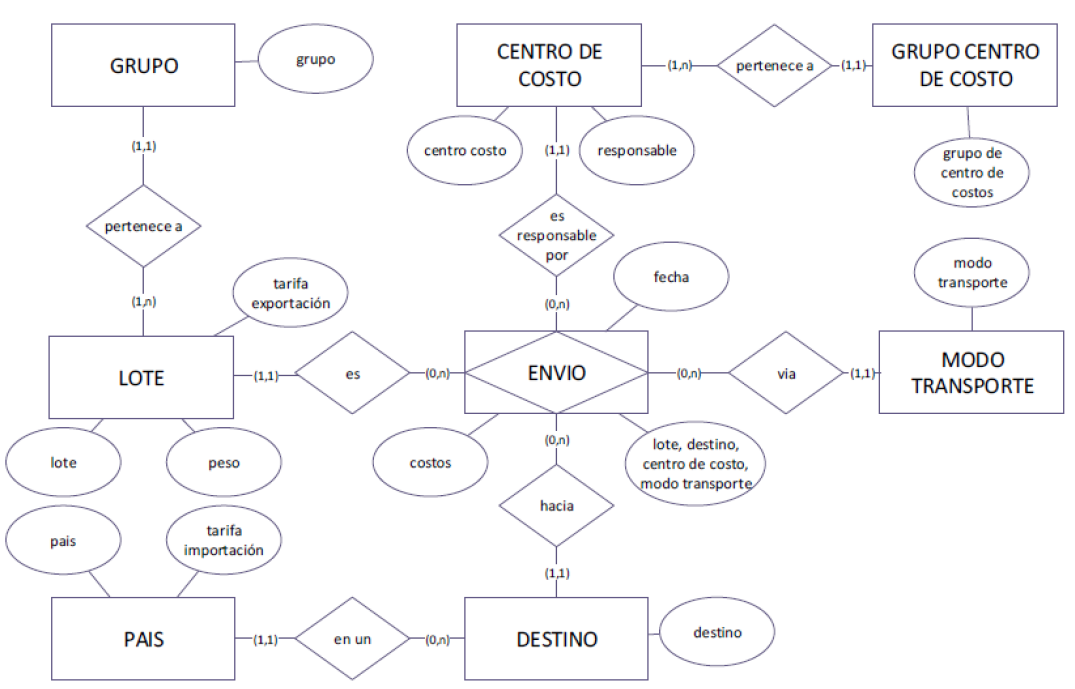
\includegraphics[width=13.5cm]{./IMAGENES/Ejercicio_1}
			%%\caption{Diagrama E/R simplificado}
		\end{center}
	\end{figure}

\subsubsection{\textbf{Modelo Dimensional }}

	\begin{figure}[htb]
		\begin{center}
			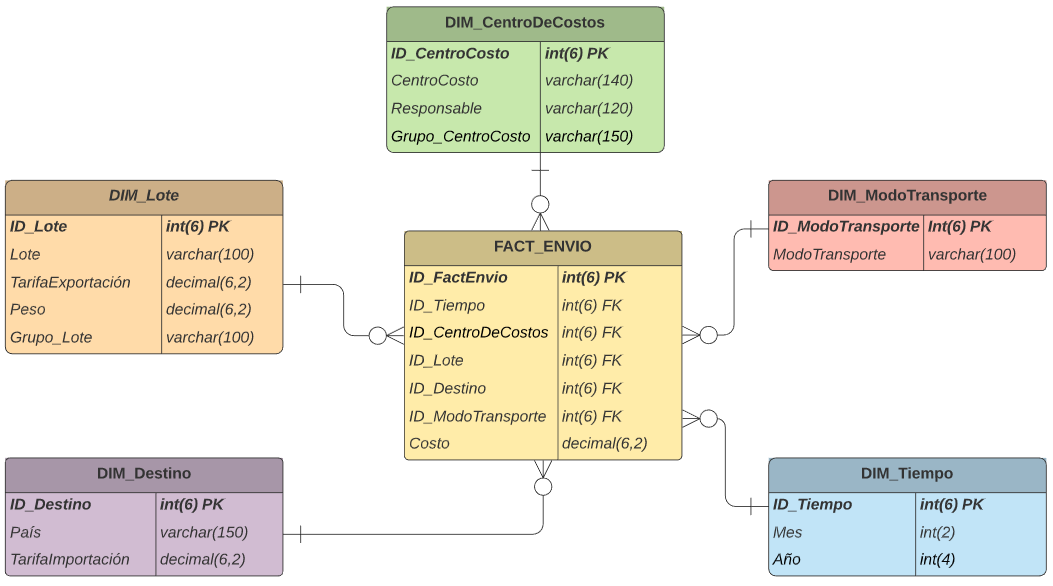
\includegraphics[width=14.5cm]{./Imagenes/mod_dimensional_1}
			%%\caption{Modelo Dimensional}
		\end{center}
	\end{figure}


%%\hfill \break
\newpage

\subsubsection{\textbf{Script SQL }}

	\begin{figure}[htb]
		\begin{center}
			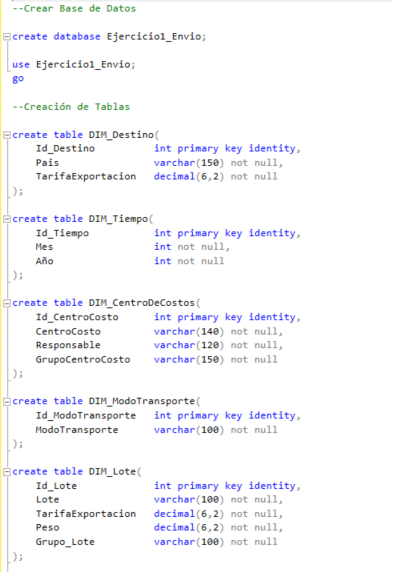
\includegraphics[width=8cm]{./Imagenes/Ejercicio1_script1}


		\end{center}
	\end{figure}

	\begin{figure}[htb]
		\begin{center}
			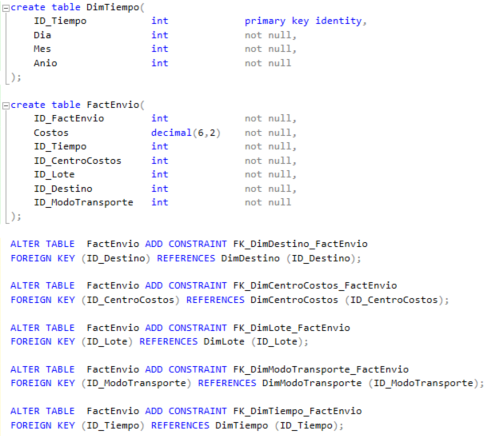
\includegraphics[width=12cm]{./Imagenes/Ejercicio1_script2}

		\end{center}
	\end{figure}



\end{document}
